\documentclass[tikz,border=10pt]{standalone}
\usepackage{tikz}
\usetikzlibrary{matrix}

\tikzset{
  cell/.style={draw=black!70, line width=1.0pt, minimum width=4.8cm, minimum height=1.15cm, align=center, text width=4.4cm, fill=none},
  head/.style={cell, draw=blue!70!black, line width=1.2pt},
  left/.style={cell, draw=green!50!black, line width=1.2pt}
}

\begin{document}
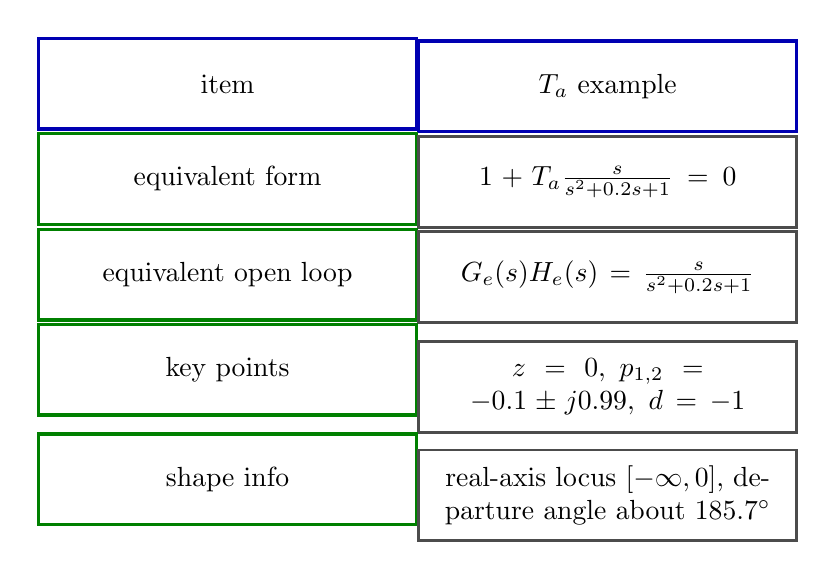
\begin{tikzpicture}
  \matrix[matrix of nodes, nodes in empty cells, row sep=-\pgflinewidth, column sep=-\pgflinewidth] {
    \node[head] {item}; &
    \node[head] {$T_a$ example}; \\
    \node[left] {equivalent form}; &
    \node[cell] {$1+T_a\frac{s}{s^2+0.2s+1}=0$}; \\
    \node[left] {equivalent open loop}; &
    \node[cell] {$G_e(s)H_e(s)=\frac{s}{s^2+0.2s+1}$}; \\
    \node[left] {key points}; &
    \node[cell] {$z=0,\ p_{1,2}=-0.1\pm j0.99,\ d=-1$}; \\
    \node[left] {shape info}; &
    \node[cell] {real-axis locus $[-\infty,0]$, departure angle about $185.7^\circ$}; \\
  };
\end{tikzpicture}
\end{document}
